\PassOptionsToPackage{force}{filehook}

\documentclass{beamer}
\usecolortheme{wolverine}
\setbeamertemplate{footline}[frame number]
%\useoutertheme{split}
%\useinnertheme{rounded}


\usepackage{pgf,tikz}
\usetikzlibrary{positioning}
\usepackage{amsmath}
\usepackage{amsfonts}
\usepackage{graphicx} 
\usepackage{subcaption}
\usepackage{hyperref}
\usepackage{cancel}
\usepackage{wrapfig}
\usepackage{comment}
\hypersetup{
	colorlinks=true,
	linkcolor=blue,
	filecolor=magenta,      
	urlcolor=cyan,
}
\newtheorem*{proposicion}{Proposici\'on}
\newtheorem*{teorema}{Teorema}
\renewcommand*{\proofname}{Demostraci\'on}
\newtheorem*{ejercicio}{Ejercicio}
\usepackage{pgf,tikz}
\usetikzlibrary{positioning}
\usepackage[spanish, activeacute]{babel} %Definir idioma español
\usepackage[utf8]{inputenc} %Codificacion utf-8
\usepackage{multirow}
\def\mydate{\leavevmode\hbox{\twodigits\day/\twodigits\month/\the\year}}
\def\twodigits#1{\ifnum#1<10 0\fi\the#1}

\title{Microeconomía}
\subtitle{Introducción\footnote{Basado en notas de Marcos Lissauer}\\ \mydate}
\author[Introducción]{Lara Sánchez Peña}


%https://tex.stackexchange.com/questions/44132/beamer-page-frame-numbers-buttons-and-appendix-slides

\date{ Universidad Torcuato di Tella}


\begin{document}

	\frame{\titlepage}
%	\let\oldmaketitle\maketitle
%\renewcommand{\maketitle}{\oldmaketitle\setcounter{footnote}{0}}

\begin{frame}{Cuestiones técnicas}
    \begin{itemize}
        \item Ver programa de la materia.
        \item Cronograma
        \item Teóricas 
        \item Prácticas
        \item Consultas
        \item Material en el campus
        \item GeoGebra - versión 5
        \item Exámenes
        \item ¿Preguntas?
    \end{itemize}
\end{frame}

\begin{frame}{Objetivo del curso}
\begin{itemize}
    \item Nos interesa entender el funcionamiento de los mercados. En particular, qué determina las transacciones que hacen los individuos y los precios de los bienes que se compran y venden.
    \item En un mercado vamos a tener: 
    \begin{itemize}
        \item Compradores - Demanda
        \item Vendedores - Oferta
    \end{itemize}
    \item Como la realidad es muy compleja, vamos a tener que analizarla a través de \textbf{modelos}. 
\end{itemize}
\end{frame}

\begin{frame}{Objetivo de la clase de hoy}
    \begin{itemize}
        \item ¿Qué es un modelo económico?
        \item Nociones sobre oferta/ demanda
        \item Curvas de oferta/ demanda
        \item ¿Qué es un quilibrio parcial o un equilibrio general?
        \item Material de repaso: Ver las slides de Eco 1 en el campus 6.2 y 6.3.
    \end{itemize}
\end{frame}

\begin{frame}{Modelos Económicos}

Un modelo es una simplificación de la realidad que nos permite estudiar ciertos fenómenos. Consiste en: 

\begin{itemize}
    \item Definiciones que describen el conjunto de variables elegidas.
    \item Supuestos. 
    \item Resultados.
\end{itemize}
\end{frame}

\begin{frame}{Modelos Económicos}
    \underline{Variables Endógenas vs Variables Exógenas}
    
    \bigskip
    
    \begin{itemize}
        \item Las \textbf{variables endógenas} son aquellas que el modelo busca explicar a partir de sus relaciones con otras variables. 
        \item Las \textbf{variables exógenas} son aquellas que están determinadas por fuera del modelo. Se toman como dadas, no se explica su comportamiento. 
    \end{itemize}
\end{frame}

\begin{frame}{Modelos Económicos}
    \underline{Supuestos}
    
    \bigskip
    
    \begin{itemize}
        \item Son proposiciones que no son objeto de análisis, pero que se dan por ciertas y de las cuales dependen los resultados del modelo. 
        \item Simplifican el mundo complejo y lo hacen más fácil de comprender.
        \item Se deja de lado lo irrelevante para el problema bajo análisis.
    \end{itemize}
\end{frame}

\begin{frame}{Modelos Económicos, por qu\'e los usamos?}
    \center\underline{{Del rigor en la ciencia}}
    \center{Jorge Luis Borges}
    \bigskip
    
    \small{\textit{... En aquel Imperio, el Arte de la Cartografía logró tal Perfección que el mapa de una sola Provincia ocupaba toda una Ciudad, y el mapa del Imperio, toda una Provincia. Con el tiempo, esos Mapas Desmesurados no satisficieron y los Colegios de Cartógrafos levantaron un Mapa del Imperio, que tenía el tamaño del Imperio y coincidía puntualmente con él. Menos Adictas al Estudio de la Cartografía, las Generaciones Siguientes entendieron que ese dilatado Mapa era Inútil y no sin Impiedad lo entregaron a las Inclemencias del Sol y de los Inviernos. En los desiertos del Oeste perduran despedazadas Ruinas del Mapa, habitadas por Animales y por Mendigos; en todo el País no hay otra reliquia de las Disciplinas Geográficas.}}
    
    \bigskip
    
    \small\textit{{Suárez Miranda, Viajes de Varones Prudentes, Libro Cuarto, Cap. XLV, Lérida, 1658.}}
\end{frame}

\begin{frame}{Modelos econ\'omicos, por qu\'e los usamos?}
\small
[...] Locke, en el siglo XVII, postuló (y reprobó) un idioma imposible en el que cada cosa individual, cada piedra, cada pájaro y cada rama tuviera un nombre propio; Funes proyectó alguna vez un idioma análogo, pero lo desechó por parecerle demasiado general, demasiado ambiguo. En efecto, Funes no sólo recordaba cada hoja de cada árbol de cada monte, sino cada una de las veces que la había percibido o imaginado. [...] %Pensó que en la hora de la muerte no habría acabado aún de clasificar todos los recuerdos de la niñez.

Los dos proyectos que he indicado (un vocabulario infinito para la serie natural de los números, un inútil catálogo mental de todas las imágenes del recuerdo) son insensatos, pero revelan cierta balbuciente grandeza. Nos dejan vislumbrar o inferir el vertiginoso mundo de Funes. Éste, no lo olvidemos, era casi incapaz de ideas generales, platónicas. %No sólo le costaba comprender que el símbolo genérico perro abarcara tantos individuos dispares de diversos tamaños y diversa forma; le molestaba que el perro de las tres y catorce (visto de perfil) tuviera el mismo nombre que el perro de las tres y cuarto (visto de frente). Su propia cara en el espejo, sus propias manos, lo sorprendían cada vez. 

[...] Había aprendido sin esfuerzo el inglés, el francés, el portugués, el latín. Sospecho, sin embargo, que no era muy capaz de pensar. Pensar es olvidar diferencias, es generalizar, abstraer. En el abarrotado mundo de Funes no había sino detalles, casi inmediatos. %La recelosa claridad de la madrugada entró por el patio de tierra.

Jorge Luis Borges, \textit{Funes el memorioso} - \href{https://www.ingenieria.unam.mx/dcsyhfi/material_didactico/Literatura_Hispanoamericana_Contemporanea/Autores_B/BORGES/memorioso.pdf}{texto completo haciendo click aqu\'i}
\end{frame}

\begin{frame}{Modelos Económicos}
    \textbf{Los modelos sirven como sustitutos de los experimentos controlados.} ¿Por qué?
    
    Se modifica una o más de las condiciones iniciales (variables exógenas, que se toman como dadas y cuyo comportamiento no se busca explicar) y se ve cómo se modifican los resultados (cómo se ven afectadas las variables endógenas). Luego, las predicciones del modelo se deben contrastar con la evidencia empírica. Ejemplo: 
    
    \begin{itemize}
        \item \textbf{Modelo}: se establece un precio máximo para el alquiler de departamentos. 
        \item Resultado del modelo (impacto que sufren las variables endógenas): se reduce la oferta de departamentos para alquilar.
        \item \textbf{Contraste empírico:} Debe observarse si efectivamente la oferta se reduce en los datos.
    \end{itemize}
\end{frame}

\begin{frame}{Modelos Económicos}
    ¿Cuáles son los factores que describen una economía en un modelo económico?
    \begin{itemize}
    \item \textbf{P}referencias
    \item \textbf{E}ndowment (dotaciones)
    \item \textbf{T}ecnología
    \end{itemize}
\end{frame}

\begin{frame}{Mercado, Consumo y Producción}
Un mercado consiste en el conjunto de compradores y vendedores de un bien o servicio. Existe un mercado para cada producto con: 
    \begin{itemize}
    \item Oferentes (productores)
    \item Demandantes (consumidores)
    \end{itemize}

    Primero vamos a estudiar por separado el comportamiento de la demanda y luego el de la oferta. Luego, encontraremos un equilibrio de mercado:
    
    
    
    \bigskip
    
    \center{\textit{Oferta $=$ Demanda $\implies$ Equilibrio de mercado}}
\end{frame}

\begin{frame}{Mercado, Consumo y Producción}

Ejemplos de \color{red}\textbf{supuestos} \color{black} que realizamos habitualmente:\footnote{Hacia el final del curso (y en OI) modificaremos estos supuestos} 

\begin{itemize}
    \item \textbf{Mercados perfectamente competitivos} que consisten de un gran
número de compradores y vendedores: las transacciones de cualquier
comprador o vendedor individual son tan pequeñas, en comparación
con el volumen total del bien o el servicio comercializado en el
mercado, que el comprador o el vendedor no tiene más remedio que
tomar el precio establecido por el mercado. \item Los consumidores y
productores gozan de \textbf{información perfecta}.
\item Hay \textbf{libre entrada y salida}
de firmas.
\end{itemize}
\end{frame}

\begin{frame}{Consumidores}
Un consumidor elige cuánto compra de cada producto, asumiendo que los precios están dados.

\textbf{Problemas:}
\begin{itemize}
    \item Hay muchos productos que los consumidores pueden comprar.
    \item Incluso considerando un solo bien, hay muchas variedades u opciones. Por ejemplo, hay diferencias de calidad para un mismo producto. 
\end{itemize}
Vamos a trabajar simplificando, abstrayéndonos de estas complejidades.

\begin{block}{Equilibrio parcial}En particular, vamos a considerar el \textbf{mercado de un solo bien}, buscaremos la demanda y la oferta de ese bien y obtendremos un \textbf{equilibrio parcial} en el mercado de ese bien. 
\end{block}
\end{frame}


\begin{frame}{Demanda}
    La demanda individual de un consumidor surge de resolver su problema de maximización de la utilidad: 
    
\begin{align*}
    \max_{{x_{1},\,x_{2}}} \,\, &u(x_{1},x_{2}) \\ &\text{s.a}: p_{1}x_{1}+p_{2}x_{2} \leq m
\end{align*}

\end{frame}

\begin{frame}{Demanda}
\begin{itemize}
    \item La cantidad demandada de un bien depende del precio: disminuye
cuando sube el precio del bien y aumenta cuando baja, dado todo lo
demás constante. Esta relación entre el precio y la cantidad
demandada es cierta para la mayoría de los bienes de la economía y es
tan general que recibe el nombre de \textbf{ley de la demanda}.
\item \textbf{Curva de demanda}: muestra cómo varía la cantidad demandada de
un bien cuando varía su precio. Nos dice a cada precio posible, la
cantidad que la gente quiere y puede comprar. Como una reducción
del precio eleva la cantidad demandada, la curva de demanda tiene
pendiente negativa.
\end{itemize}
\end{frame}


\begin{frame}{Demanda}
\begin{itemize}
    \item La \textbf{curva de demanda} se refiere a la demanda agregada, que se obtiene
de sumar, para cada precio posible, las cantidades que quieren comprar
todos los potenciales compradores:
\[
D(p) = \sum_{i=1}q_{i}^{d}(p), \quad \forall \, p
\]
\end{itemize}

\begin{figure}
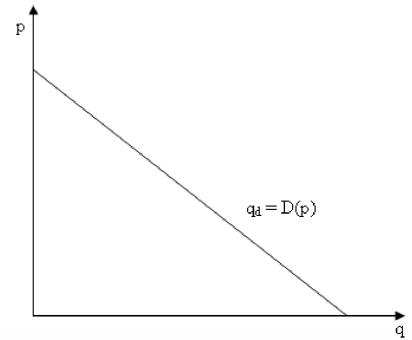
\includegraphics[width=5.5cm]{figures1/demand.png}
\end{figure}
\end{frame}

\begin{frame}{Demanda}
Es importante tener en cuenta que en el gráfico previo suponemos
implícitamente que cualquier variable que pueda afectar la demanda,
permanece constante. ¿Cuáles son algunas de estas otras variables que
determinan la demanda?

\begin{itemize}
    \item Ingreso de los consumidores.
    \item Preferencias de los consumidores.
    \item Precio de bienes sustitutos o complementarios.
\end{itemize}

\textbf{Importante:} El cambio en el precio del bien en cuestión, causa un
\textbf{movimiento a lo largo de la curva de demanda} (cambio en la cantidad demandada, no en la función). Un cambio en cualquier otro factor que no esté en los ejes causa un
\textbf{desplazamiento de la curva de demanda} (cambio en la demanda). 
\end{frame}

\begin{frame}{Demanda: ejemplo}
    \begin{itemize}
        \item Supongamos que Emma y Fede tienen las siguientes \textbf{funciones de demanda} para comprar alfajores: 
        
    \begin{align*}
        &Q^{d}_{Fede}(p) = 10-2p \quad \quad \text{si} \, p \leq 5\\
        &Q^{d}_{Emma}(p) = 5-p  \,\,\, \quad \quad \text{si} \, p \leq 5
    \end{align*}
    \end{itemize}
\end{frame}

\begin{frame}{Demada: ejemplo}
   \begin{itemize}
       \item La demanda agregada resulta:
       
\begin{align*}
    &Q_{agregada}^{d}(p) = Q^{d}_{Fede} + Q^{d}_{Emma}\\
    &Q_{agregada}^{d}(p) = 15 - 3p
\end{align*}
    \item Para graficar, buscamos la curva de demanda agregada inversa: 
\begin{align*}
    P_{agregada}^{d}(Q) = 5-\frac{1}{3}Q
\end{align*}
   \end{itemize} 
\begin{figure}
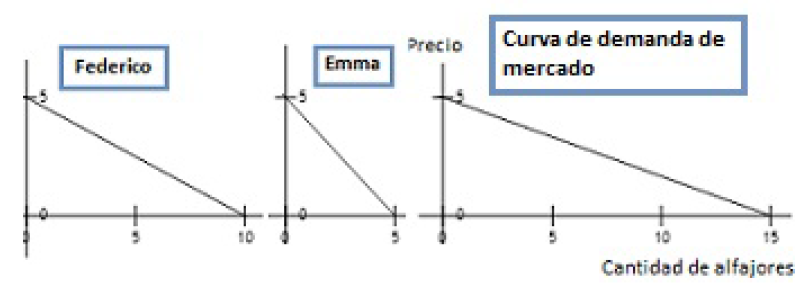
\includegraphics[width=10cm]{figures1/demanda_alfajores.png}
\end{figure}
\end{frame}   

\begin{frame}{Demanda: ejemplo}
    \begin{itemize}
        \item Supongamos que en el mercado de este bien se agrega una consumidora más: Cata. 
        \item La función de demanda de Cata es: 
        \[Q_{Cata}^{d}(p) = 3 - p\]
        \item Por lo tanto, ahora la demanda agregada es la suma de lo que demandan los tres consumidores: 
\begin{align*}
    Q^{d}_{Fede} &= 10-2p \quad \quad \text{si} \, p\leq 5\\
    Q^{d}_{Emma} &= 5-p \quad \quad \,\,\, \text{si}\, p\leq 5\\
    Q^{d}_{Cata} &= 3-p \quad \quad \,\,\, \text{si} \, p\leq 3
\end{align*}
        \item Pero en este caso las funciones de demanda están definidas
        para distintos rangos de precios, por lo que es necesario
        separar la demanda agregada por tramos.
    \end{itemize}
\end{frame}

\begin{frame}{Demanda: ejemplo}
\begin{align*}
    Q_{agregada}^{d}(p) = \begin{cases}
    Q_{Fede}^{d}(p) + Q_{Emma}^{d}(p)+Q_{Cata}^{d}(p) & \text{si} \, p\leq 3\\
    Q_{Fede}^{d}(p) + Q_{Emma}^{d}(p) & \text{si} \, 3<p\leq 5\\
    0 & \text{si} \, p> 5
    \end{cases}
\end{align*}
Para precios mayores a 5 ni Fede ni Emma ni Cata demandan
alfajores, si el precio está entre 3 y 5 solamente Fede y Emma
quieren comprar alfajores y, si el precio es menor o igual a 3, todos
demandan alfajores.
\begin{align*}
    Q_{agregada}^{d}(p) = \begin{cases}
   18-4p & \text{si} \, p\leq 3\\
    15-3p & \text{si} \, 3<p\leq 5\\
    0 & \text{si} \, p> 5
    \end{cases}
\end{align*}
\end{frame}

\begin{frame}{Demanda: ejemplo}
Para graficar de la forma en la que estamos acostumbrados,
obtenemos la demanda agregada inversa para cada uno de los
tramos.

\begin{align*}
    P_{agregada}^{d} (Q)=\begin{cases}
    4,5 - \frac{1}{4}Q & \text{si} \,\, 6 \leq Q \leq 18\\
    5-\frac{1}{3}Q & \text{si} \,\, 0\leq Q\leq 6
    \end{cases}
\end{align*}

\begin{figure}
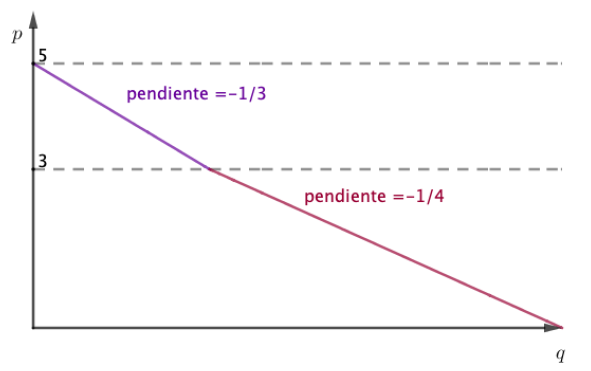
\includegraphics[width=7.5cm]{figures1/demand_3.png}
\end{figure}
\end{frame}

\begin{frame}{Oferta}
\begin{itemize}
    \item \textbf{Curva de oferta:} relaciona el precio de un producto con la cantidad
    que las firmas desean producir y vender. La forma de la curva de
    oferta resulta de las decisiones de la firma. 
    \item La oferta individual de cada firma surge del problema de \textbf{maximización de beneficios}:
    
    \begin{align*}
        \max_{q} \, &\pi = \underbrace{ p \cdot q}_{IT} - \underbrace{C(q)}_{CT}
    \end{align*}
    
    \item \textbf{Ley de oferta:} las firmas están dispuestas a producir y vender más de un bien cuando su precio aumenta.
\end{itemize}
\end{frame}

\begin{frame}{Oferta}
    \begin{itemize}
        \item Esta curva de oferta se refiere a la oferta agregada, que se obtiene de sumar, para cada precio posible, las cantidades que quieren vender todos los potenciales productores.
        
        \[S(p) = \sum_{j}q_{j}^{s}(p), \,\, \forall \, p
        \]
    \end{itemize}
    
\begin{figure}
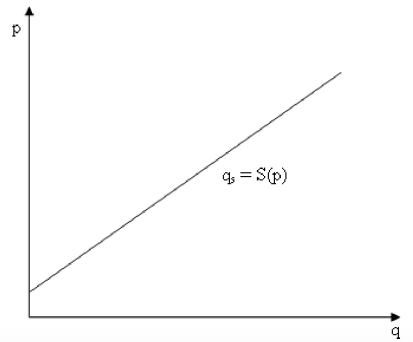
\includegraphics[width=5.5cm]{figures1/supply.png}
\end{figure}
\end{frame}

\begin{frame}{Oferta}
Es importante tener en cuenta que en el gráfico previo suponemos implícitamente que cualquier variable que pueda afectar la oferta, permanece constante. ¿Cuáles son algunas de estas otras variables que
determinan la oferta?
\begin{itemize}
    \item Tecnología.
    \item Número de productores.
    \item Precio de los insumos 
    \item Factores aleatorios (ej: clima)
\end{itemize}
\textbf{Importante:} El cambio en el precio del bien en cuestión, causa un
\textbf{movimiento a lo largo de la curva} de oferta (cambio en la cantidad ofrecida, no en la función). Un cambio en cualquier otro factor que no esté en los ejes causa un \textbf{desplazamiento de la curva} de oferta (cambio en la oferta).
\end{frame}

\begin{frame}{Equilibrio parcial}
En equilibrio, en un mercado perfectamente competitivo de un bien se establecerá un precio
y una cantidad de manera que no haya un exceso de oferta ni un exceso de
demanda, por lo tanto, \textbf{la demanda es igual a la oferta para un precio de equilibrio}:

\[
D(p^*) = S(p^*)
\]

\begin{itemize}
    \item Si existe un exceso de oferta a un precio $p$, $S(p)>D(p)$, $\implies$ el precio debería caer.
    \item Si existe un exceso de demanda a un precio $p$, $S(p)<D(p)$, $\implies$ el precio debería aumentar.
\end{itemize}
\end{frame}

\begin{frame}{Equilibrio parcial}
\begin{figure}
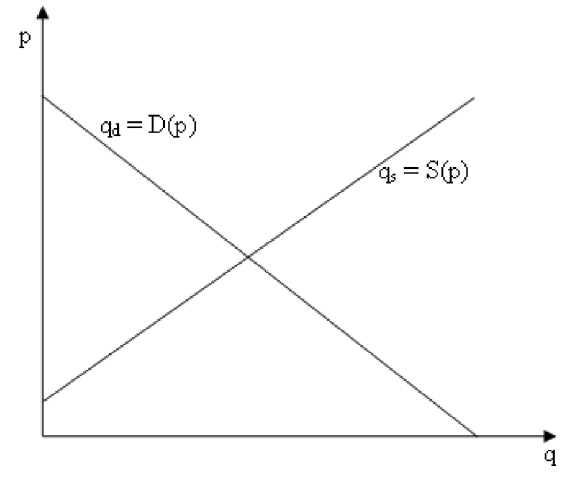
\includegraphics[width=7.5cm]{figures1/equilibrium.png}
\end{figure}
\end{frame}

\begin{frame}{Equilibrio parcial}
    El \textbf{equilibrio de mercado} se define como $(q^{*},p^{*})$: una cantidad de mercado $q^{*}$ y un precio de mercado $p^{*}$ que cumplan que la cantidad demandada y cantidad ofrecida a a ese precio sean iguales, es decir, 
    \[D(p^{*}) = S(p^{*}).\]
    
    \begin{itemize}
        \item Los compradores determinan conjuntamente la \textbf{demanda} del producto y los vendedores, la \textbf{oferta}.
        \item Como vimos, los determinantes de la demanda son estudiados por la \textbf{teoría del consumidor}, mientras que los de la oferta son estudiados por la \textbf{teoría de la firma}.
        \item El equilibrio surge de entre la interacción entre la \textbf{demanda} y la \textbf{oferta}.
        \item El equilibrio, ¿es \textbf{estable}?
    \end{itemize}
\end{frame}

\begin{frame}{Equilibrio parcial vs. Equilibrio general}
    \begin{itemize}
\item    Cuando se hace un análisis de  \textbf{equilibrio parcial} se estudia qué ocurre en el mercado de un bien. Se consideran los cambios en este mercado aisladamente, es decir, por separado de lo que ocurre en otros mercados, considerando que en los demás mercados no hay cambios que afecten significativamente al mercado que se está analizando.
    
 \item   Cuando se hace un análisis de \textbf{equilibrio genera}l se estudia no sólo qué cambios ocurren dentro de cada mercado, sino también como éstos afectan a otros mercados.
 
 \vspace{6pt}
 \underline{Por ejemplo:} mercado de petróleo, viajes en avión, comestibles, energía solar...
    
 \end{itemize}   
\end{frame}

\begin{frame}{Equilibrio de corto plazo vs. largo plazo}
    Podríamos considerar equilibrios de \begin{itemize}
        \item \textbf{corto plazo}: hay insumos cuya cantidad (por ejemplo, $K$) está fija y eso genera \textbf{costos fijos}, \textbf{la cantidad de firmas está dada}, las firmas pueden decidir \textbf{producir o no producir}.
        \item \textbf{largo plazo}:  las firmas pueden elegir cualquier combinación de insumos (por ejemplo, $L$ y $K$) por lo que \textbf{no hay costos fijos}, hay libre entrada de firmas (las firmas pueden decidir si \textbf{salir o no del mercado}).
        
        \begin{block}{Recordar:}
 El concepto de (corto y largo) plazo está relacionado con las elecciones que pueden tomar las firmas.

Por lo tanto, un equilibrio de largo plazo consiste de $(p^*,q^*,n^*)$, donde $n^*$ representa la cantidad de firmas.
        \end{block}
    \end{itemize}
\end{frame}
\end{document}

